\section{Player Motivation}
\label{chap:player_motivation}
In this chapter, we will continue presenting results from the study relevant to \textit{RQ3: “How do game design elements and social interaction affect the players’ motivation in our game concept?”}. Results from the questionnaire, interviews, and observations of participants will be described.

\subsection{Questionnaire}
The questionnaire includes ten statements and three questions related to the players’ motivation, presented in Table \ref{tab:motivation_statements} below. Similar to the previous chapter, a three-point Likert scale is used. Averages for the student society (Avg S) and classmates (Avg C) group are also included.

\begin{table}[H]
    \hspace*{-0.015\textwidth}
    \begin{tabularx}{1.03\textwidth}{|c|X|c|c|c|c|c|}
        \hline
        & \multicolumn{1}{c|}{\textbf{Statements}}  & \multicolumn{1}{c|}{\textbf{Disagree}} & \multicolumn{1}{c|}{\textbf{Neutral}}  & \multicolumn{1}{c|}{\textbf{Agree}} & \multicolumn{1}{c|}{\textbf{Avg S}} & \multicolumn{1}{c|}{\textbf{Avg C}}\\ \hline
        \textbf{S7} & I was motivated to carry out activities by the opportunity to win medals. & 57.9\% & 10.5\% & 31.6\% & 2.33 & 3.29 \\
        \textbf{S8} & I was motivated to carry out activities by the opportunity to earn points. & 15.8\% & 5.3\% & 79.0\% & 3.50 & 4.29 \\
        \textbf{S9} & I was motivated to carry out activities because others did it & 15.8\% & 10.5\% & 73.7\% & 3.75 & 3.71 \\
        \textbf{S10} & was motivated to carry out activities to keep my streak alive. & 57.9\% & 21.1\% & 21.1\% & 2.25 & 2.71 \\
        \textbf{S11} & Reactions to my activities inspired me to use the application more. & 63.2\% & 21.1\% & 15.8\% & 1.92 & 3.14 \\
        \textbf{S12} & The leaderboard motivated me to get as many points as possible. & 0.0\% & 15.8\% & 84.2\% & 4.17 & 4.43 \\
        \textbf{S13} & The ability to earn double points by using the application with a friend inspired me to use it more. & 10.5\% & 5.3\% & 84.2\% & 4.58 & 3.57 \\
        \textbf{S14} & Challenges between friends inspired me to use the application. & 15.8\% & 10.5\% & 73.7\% & 3.42 & 4.29 \\
        \textbf{S15} & I was inspired to use Hover by other players' activities. & 21.1\% & 15.8\% & 63.2\% & 3.25 & 3.57 \\
        \textbf{S16} & I opened the application when I received a notification. & 73.7\% & 5.3\% & 21.1\% & 2.33 & 2.43 \\
        \hline
    \end{tabularx}
    \caption{Statements related to motivation.}
    \label{tab:motivation_statements}
    \vspace*{-2\baselineskip}
\end{table}

As seen in the table, most of the answers are gathered in the “disagree” or “agree” alternative. The “neutral” option is never above 21.1\%.

Based on the answers, there were mainly three elements that seemed to have less effect on increasing the players’ motivation. Only 31.6\% agreed that winning medals (S7) increased their motivation for playing the game. The inclusion of streaks (S10) and the possibility of reacting to posts in the feed (S11) did not either increase the players’ motivation. Additionally, the last statement (S16) revealed that notification seemed to have a limited influence on the use of the application. Almost three-quarters answered that they did not open the application when they received a notification.

On the other side, six of the game elements had a motivating effect. Earning points (S8) and influence from friends (S9) positively impacted the participants’ motivation. However, the possibility for users to view their position in a leaderboard (S12), and get double points when hovering together with a friend (S13),  seemed to have the highest impact. As much as 84.2\% percent of the participants agreed that these affected their motivation. In addition to these aspects, challenges between friends (S14) and the ability to follow other people’s activities in the feed (S15) positively influenced the players’ motivation. 

As mentioned above, the table also includes the average results for the two test groups. The classmates (group C) had a generally higher average than the student society (group S). The only question where the answers from the student society group had a higher average was in S13.

As described at the beginning of this subsection, four questions (Table \ref{tab:motivation_questions}) were asked to the participants. The results from the first three are presented in Figure \ref{fig:motivation_questions}. 

\begin{table}[H]
    \centering
    \begin{tabularx}{\textwidth}{|c|X|}
        \hline
        & \multicolumn{1}{c|}{\textbf{Questions}} \\ \hline
        \textbf{Q16} & How often during the test period were you inspired by your friends to use Hover? \\
        \textbf{Q17} & How often during the test period were you inspired by challenges to using Hover? \\
        \textbf{Q18} & How often during the test period were you inspired by medals to use Hover? \\
        \hline
    \end{tabularx}
    \caption{Questions related to motivation.}
    \label{tab:motivation_questions}
    \vspace*{-\baselineskip}
\end{table}

\begin{figure}[H]
    \centering
    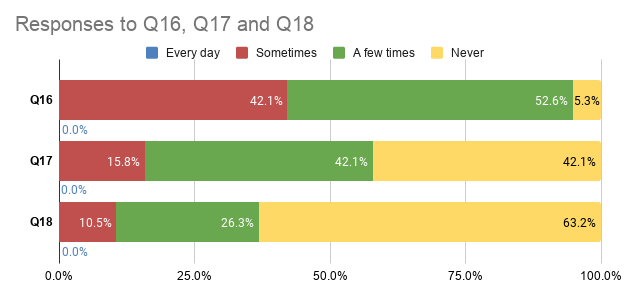
\includegraphics[width=0.97\textwidth]{Images/Results/Motivation/MotivationQuestions.png}
    \caption{Answers to questions related to motivation.}
    \label{fig:motivation_questions}
\end{figure}

The questions give more insight into how often the users were motivated by friends (Q16), challenges (Q17), and achievements (Q18). The first question confirms the answers in S12 and S13, proposing that the social aspect of Hover motivates the players. The last question also (Q18) coincides with the associated statement (S7). The participants were not particularly inspired by the possibility to earn achievements.

\begin{wrapfigure}{r}{0.5\textwidth}
    \hspace*{-0.1\textwidth}
    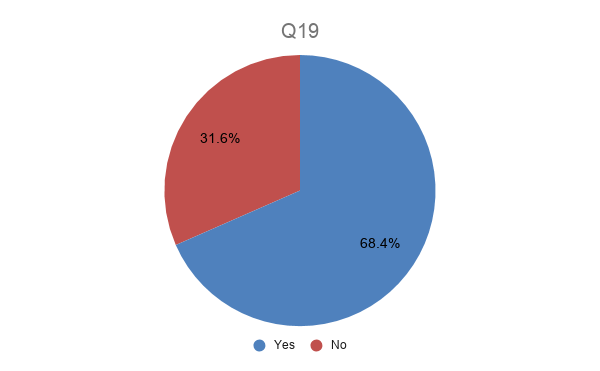
\includegraphics[width=0.7\textwidth, left]{Images/Results/Motivation/PointsVsEffort.png}
    \caption{Answers to questions related to motivation.}
    \label{fig:correct_points}
    \vspace*{-\baselineskip}
\end{wrapfigure}

In question Q17, 84.22\% of the participants answered that they were not never or only a few times motivated by challenges to use Hover. This result can be seen as a bit conflicting with statement S14, where 73.88\% agreed that challenges between friends motivated them.

Additionally, the next question (Q19) asked the participants, “Was the number of points in each category correct in relation to your effort?”. As seen in Figure \ref{fig:correct_points}, two-thirds of the players thought the points were distributed fairly. The people responding “No” to this question mentioned that the points awarded in the culture zones should have been lower:

\textit{“The educational points were a bit too low, compared to culture.”\footnotemark[\value{footnote}]}

\textit{“A bit too many points to collect at Samfundet (culture category)”\footnotemark[\value{footnote}]}

\textit{“Somewhat demotivating that you got a lot more points for culture than school”\footnotemark[\value{footnote}]}

At the end of the motivation part of the questionnaire, the participants were allowed to write additional comments or feedback they might have. These questions gave us multiple positive reactions to the concepts:

\textit{“Very cool concept that I will continue to use to motivate me to go to school”\footnotemark[\value{footnote}]}

\textit{“The challenges motivated me to go to school”\footnotemark[\value{footnote}]}

\textit{“A very cool concept with a lot of potentials”\footnotemark[\value{footnote}]}

\footnotetext{Translated from Norwegian}

\subsection{Interviews}
In the interviews, we got some more feedback on which elements of the game motivated the players. The data confirmed the results obtained in the questionnaire, but we also got some additional reactions and perspectives.

All the participants mentioned points and friends as essential motivation factors. While these answers were in line with the results from the questionnaire, other ones did not correspond that well. An example of that was the leaderboard which could be perceived as less motivating. As mentioned in the questionnaire section above, some of the participants expressed that the number of points sometimes was distributed unfairly. Consequently, the distance between participants in the leaderboard could become substantial, decreasing the motivation for some players.

\textit{“In the first 3-4 days, I did not get a lot of points. After that it was already so far up to the top of the leaderboard, that my motivation decreased.”\footnotemark[\value{footnote}]}

\footnotetext{Translated from Norwegian}

The response to challenges between friends was also mixed. Some users described them as motivating, while others did not feel the same way. One of the participants said:

\textit{“When I was invited to challenges, I felt I had to get to school to use the app to win. It was motivating.”\footnotemark[\value{footnote}]}

Another one mentioned that the challenges would become more fun if the rules were not as customizable. By allowing everyone to set their own rules for the challenges, people could create one they were sure to win themselves. Making it less fun for others.

\textit{“The challenges did not work as well for me. Because if I were to make one, I would be sure that I made one that I was certain to win. [...] It would probably be better to not make them as customizable.”\footnotemark[\value{footnote}]}

Another proposal for enhancing the player’s motivation was to add more incentives for earning points. One of the participants suggested that adding some sort of real-life rewards in exchange for points would increase the motivation for hovering. Another participant wished they could use their score on in-game elements.

\textit{“The rewards did not give me sufficient incentive for playing. [...] I think I would have been more motivated if I could spend it on something in the cafeteria.”\footnotemark[\value{footnote}]}

\textit{“I wish I could use the score to buy background color in the app or a cooler hat for my avatar. Such things work very well for me.”\footnotemark[\value{footnote}]}

\subsection{Observations}
Observations of participants playing the game again confirmed how important the social aspect was for the motivation. There were multiple situations of someone mentioning the game to others, sometimes almost forcing them to play. Without the social incentive and pressure to play, players’ motivation would decrease. Apart from this confirmation, the observations did not reveal anything worth mentioning.

\subsection{Summary}
The aspect of the survey related to the players’ motivation has been presented in this chapter. In the next one, we will shift focus to the players’ enjoyment and look at data that can be used to answer the next research question, RQ4.

